\chapter{Introduction}\label{Introduction}
%%%%%%%%%%%%%%%%%%%%%%
% Was wurde untersucht? Was ist daran neu?
% Warum ist das schwierig? Was sind die Herausforderungen?
% Warum relevant?
% Was leistet meine Arbeit? Welche wiss. Beiträge leiste ich?
% Was gibt es für ähnliche Arbeiten? Wie ist meine Anders?
% Der Fahrplan: Wie ist die Arbeit aufgebaut?
%%%%%%%%%%%%%%%%%%%%%%

%    What is the problem?
%    Why is it interesting and important?

Recursion is concise and easy to understand and write, since it resembles our inductive way of thinking about recursive tasks. We start from a nonrecursive basecase and then construct the recursive cases. The problem with recursion in general is, that each recursive call adds a layer on the callstack of the operating system. Adding a new layer on the callstack is incredibly exepnsive in terms of time and memory. All variables, returning addresses etc. pp. need to be copied to the stack when switching the context, and restored when popping the layer. Therefore, computation is not limited by time, but limited by memory. Due to the (in general) exponential callstacks growth, most recursive functions are impractical for many real world problems.

%    Why is it hard? (E.g., why do naive approaches fail?)
Iterative solutions with dynamic programming are usually the way to go where recursion is impractical. By iterartivly manipulating a fixed amount of memory, the memory consumption is limited and expensive context switches are avoided. Translating an unbounded, problem oriented, imperformant algorithm into an imperative language like Java and implementing dynamic programming can be quite challanging. If you can even exploit specific mathematical properties of the problem to constraint the search space, you are in luck. But this is a time consuming task and developer time is always a very limited resource. If your target language is not imperative but declarative like SQL, you will additionally need a decent amount of knowledge of SQL, the query planner and probably other internals of the database system to come up with a performant solution to your recursive problem.

%    Why hasn't it been solved before? (Or, what's wrong with previous proposed solutions? How does mine differ?)
What would we loose, if we decide to write a function over vast amounts of data not in SQL but in, say Java, because it is easier to write fairly performing implementation than in SQL.
....
So there is a good point to do as much computations as possible right in the database.




\paragraph*{Running example}

\begin{wrapfigure}{r}{0.5\textwidth}
  \vspace{-20pt}
    \sqlcode{snippets/fib.sql}
  \caption{SQL UDF returning the nth Fibonacci number}
  \label{intro_fib}
\end{wrapfigure}


The Fibonacci function will serve us as guinea pig in this introductiary example and throughout the thesis.
It is defined as $F_n = F_{n-1} + F_{n-2}$ with $F_0 = 0$ and $F_1 = 1$. There are various ways of defining this
function as SQL UDF, but in this example we will use the (slightly awkward) formulation from figure \autoref{intro_fib}.

What happens if we call \mintinline{postgresql}{SELECT fib(4)}? The planner takes some time to have a close look at the query inside fib to make an execution plan and then executes this plan. During execution, a number of subcalls occurs that need to be executed before the surrounding query can be evaluated. Everytime, the UDF is replanned and a callstack will grow as illustrated in \autoref{fib_4_callstack}. As soon as a node has the result of all of its children, the node can itself return a result. The leaves of the tree can therefore return a result immediately and the evaluation starts bottom-up (\autoref{fib_4_callstack_evaluation}). 

The idea behind the translation is to simulate this two phases: top-down callstack-growth and bottom-up evaluation. To generate the callstack we need to keep track of subsequent calls. To achieve this, we slice the UDF into all possible evaluation scenarios together with predicates to test if a scenario is executed with the current arguments. Now, we can evaluate the \textit{arguments} of the callsites of the current scenario and add subseqent calls to the callstack by this. Substituting the original call arguments (eg. \texttt{\$1} or \texttt{n}) with a reference to the newly discovered arguments from the previous iteration, we are able to generate a complete callstack.

Evaluation starts from the bottom: The leaves of the the callstack do not contain any callsites and can therefore evaluated directly. From here evaluation ascends the callstack again and callsites are replaced with references to their values inside the evaluation-table. As soon as all callsites of a scenario have a result available, the scenario can be evaluated and the result is added to the evaluation table. This continues until we can compute the final result.

\paragraph*{Structure of this thesis}
There are two interesting parts regarding the translation. The first is the template itself and its various optimizations that can be applied under certain circumstances, eg. when the function is tail recursive. The other interesting part is how to derive the sliced representation of the UDF that is used to fill the templates. I provide a small-step operational semantics over a subset of SQL:1999 to compile a query into its scenarios.
My thesis digs deep on the latter and just flys over the templates, since the templates were provided by my supervisor and it was mainly my task to develop the formal inference rules and implement them in Haskell.

%The idea of the callstack CTE is to collect in every step the arguments of the newly occuring recursive calls. With the data of the analysis, this is a simple task. The following pseudocode gives you an intuition: \mintinline{postgresql}{SELECT in_args, callsite.id, callsite.args FROM scenario.pred p WHERE p.v}. This snippet returns the arguments of a callsite within a scenario that is called with the given \texttt{in\_args} if the predicate of the scenario evaluates to true. If we do this for every callsite in every scenario, we receive a complete level in the tree of the callstack (see \autoref{discovery_strucutre}). To compute the complete callstack, we need to iterate over every set of arguments from the previous call (ie. the level above) and continue collecting calls until no new calls are outputed since we reached the basecases. See \autoref{callstack_recurse} for an illustration.

\begin{figure}
    \begin{minipage}[b]{.5\linewidth}
        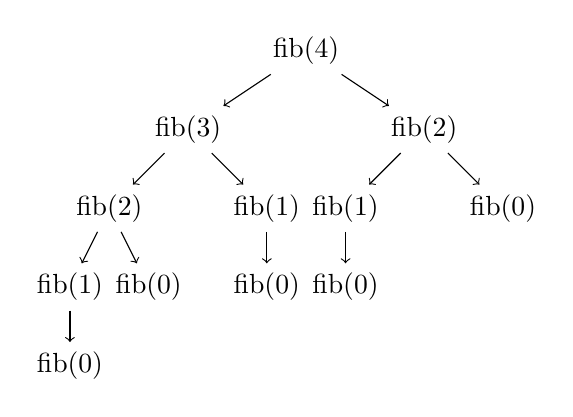
\begin{tikzpicture}
        % nodes
        \node (n1)     at (2.5, 2) {fib(4)};
            \node (n1-1)   at (1, 1) {fib(3)};
                \node (n1-1-1) at (0, 0) {fib(2)};
                    \node (n1-1-1-1) at (-0.5, -1) {fib(1)};
                        \node (n1-1-1-1-0) at (-0.5, -2) {fib(0)};
                    \node (n1-1-1-2) at (0.5, -1) {fib(0)};
                \node (n1-1-2) at (2, 0) {fib(1)};
                    \node (n1-1-2-0) at (2, -1) {fib(0)};
            \node (n1-2)   at (4, 1) {fib(2)};
                \node (n1-2-1) at (3, 0) {fib(1)};
                    \node (n1-2-1-0) at (3, -1) {fib(0)};
                \node (n1-2-2) at (5, 0) {fib(0)};
        % arrows
        \draw[->] (n1)     -- (n1-1);
        \draw[->] (n1)     -- (n1-2);
        \draw[->] (n1-1)   -- (n1-1-1);
        \draw[->] (n1-1)   -- (n1-1-2);
        \draw[->] (n1-2)   -- (n1-2-1);
        \draw[->] (n1-2)   -- (n1-2-2);
        \draw[->] (n1-1-1) -- (n1-1-1-1);
        \draw[->] (n1-1-1) -- (n1-1-1-2);
        \draw[->] (n1-1-1-1) -- (n1-1-1-1-0);
        \draw[->] (n1-1-2) -- (n1-1-2-0);
        \draw[->] (n1-2-1) -- (n1-2-1-0);
        \end{tikzpicture}
        \caption{Growth of the callstack of \texttt{fib(4)}}
        \label{fib_4_callstack}
    \end{minipage}
    \begin{minipage}[b]{.5\linewidth}
        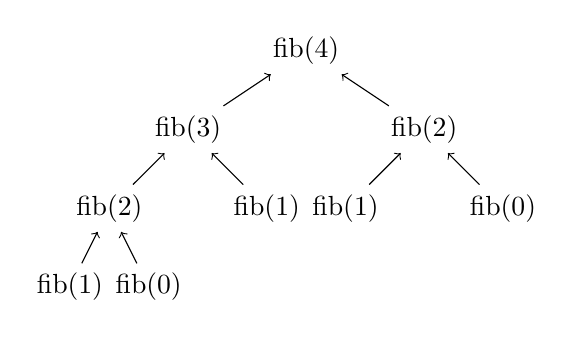
\begin{tikzpicture}
        % nodes
        \node (n1)     at (2.5, 2) {fib(4)};
        \node (n1-1)   at (1, 1) {fib(3)};
        \node (n1-1-1) at (0, 0) {fib(2)};
        \node (n1-1-1-1) at (-0.5, -1) {fib(1)};
        \node (n1-1-1-2) at (0.5, -1) {fib(0)};
        \node (n1-1-2) at (2, 0) {fib(1)};
        \node (n1-2)   at (4, 1) {fib(2)};
        \node (n1-2-1) at (3, 0) {fib(1)};
        \node (n1-2-2) at (5, 0) {fib(0)};
        % arrows
        \draw[<-] (n1)     -- (n1-1);
        \draw[<-] (n1)     -- (n1-2);
        \draw[<-] (n1-1)   -- (n1-1-1);
        \draw[<-] (n1-1)   -- (n1-1-2);
        \draw[<-] (n1-2)   -- (n1-2-1);
        \draw[<-] (n1-2)   -- (n1-2-2);
        \draw[<-] (n1-1-1) -- (n1-1-1-1);
        \draw[<-] (n1-1-1) -- (n1-1-1-2);
        \end{tikzpicture}
        \caption{Evaluation of the callstack of \texttt{fib(4)}}
        \label{fib_4_callstack_evaluation}
    \end{minipage}
\end{figure}

By collecting all calls in a table it is also trivial to remove duplicate calls from the callstack before evaluation (figure z), which gives us memoization which speeds up the translation significantly. The callstack table is just a relational representation of the callstack with memoization (Table T).


Translation begins with a static analysis that compiles the \CASE-expression into standalone predicates and queries (\autoref{fib_analysis_output}). Note how the predicates include the negation of the leading predicates. Beside cutting the UDF into slices the analysis also enumerates the callsites contained in the given scenario. For each callsite the arguments are extracted as standalone queries with only the UDF arguments as free variables. This data is used to do the macro expansion that generate the translated UDF. Chapter \autoref{approach} explains the ins and outs of the inference rules of the static analysis, but in this introduction I continue with the templates and how they work.



\begin{figure}
    \begin{minipage}[b]{.5\linewidth}
    \centering
        \begin{align*}                                    \\
         &\langle~&\text{pred}: ~&\mintinline{postgresql}{SELECT ($1 = 0)}                  ,\\
         &        &\text{query}:~&\mintinline{postgresql}{SELECT 0}                         \rangle\\
        \end{align*}
    \subcaption{Nonrecursive scenarios}\label{fib_nonrec_scenarios}
    \end{minipage}%
    \begin{minipage}[b]{.5\linewidth}
    \centering
        \begin{align*}
        &\big\langle~&\text{pred}:~ &\mintinline{postgresql}{SELECT (NOT $1 = 0) AND ($1 = 1)}  ,\\
        &            &\text{query}:~&\mintinline{postgresql}{SELECT 1 + fib(0)},     \\
        &            &\text{callsites}:~&\langle \text{id}: 1,~\text{args}: (\mintinline{postgresql}{SELECT 0})\rangle\big\rangle,\\
        &\big\langle&\text{pred}:~ &\mintinline{postgresql}{SELECT (NOT $1 = 0) AND (NOT $1 = 1)}  ,\\
        &           &\text{query}:~&\mintinline{postgresql}{SELECT fib($1 - 1) + fib($1 - 2)},     \\
        &           &\text{callsites}:~&\langle \text{id}: 2,~\text{args}: (\mintinline{postgresql}{SELECT $1 - 1})\rangle, \\
        &           &                  &\langle \text{id}: 3,~\text{args}: (\mintinline{postgresql}{SELECT $1 - 2})\rangle\big\rangle\\
        \end{align*}
    \subcaption{Recursive scenarios}\label{fib_rec_scenarios}
    \end{minipage}
    \caption{Output of scenario analysis of \mintinline{postgresql}{fib(int)} from \autoref{intro_fib}}\label{fib_analysis_output}
\end{figure}

        
\begin{figure}
    \centering
            \bgroup
            \def\arraystretch{1.5}
        \begin{tabular}{|c|}\hline
            %\footnotesize\mintinline{postgresql}{in_args := $1 / SELECT c.call_args FROM callstack c}\\
            \begin{tabular}{|l|}\hline
                \footnotesize{Scenario 1}\\
                \begin{tabular}{|l|}\hline
                    \footnotesize{Callsite 1}\\
                    \footnotesize\mintinline{postgresql}{SELECT in_args, callsite.id, callsite.args AS call_args}\\[-5pt]
                    \footnotesize\mintinline{postgresql}{  FROM scenario.pred p WHERE p.v}\\
                \hline \end{tabular}\\
                \mintinline{postgresql}{UNION}\\
                \begin{tabular}{|l|}\hline
                    \footnotesize{Callsite 2}\\
                    \footnotesize\mintinline{postgresql}{SELECT in_args, callsite.id, callsite.args AS call_args}\\[-5pt]
                    \footnotesize\mintinline{postgresql}{  FROM scenario.pred p WHERE p.v}\\
                \hline \end{tabular}\\[2mm]
            \hline \end{tabular}\\
                \mintinline{postgresql}{UNION}\\
            \begin{tabular}{|l|}\hline
                \footnotesize{Scenario 2}\\
                \begin{tabular}{|l|}\hline
                    \footnotesize{Callsite 3}\\
                    \footnotesize\mintinline{postgresql}{SELECT in_args, callsite.id, callsite.args AS call_args}\\[-5pt]
                    \footnotesize\mintinline{postgresql}{  FROM scenario.pred p WHERE p.v}\\
                \hline \end{tabular}\\[2mm]
            \hline \end{tabular}
            \\[6mm]
        \hline
        \end{tabular}
        \egroup
    \caption{Structure of the callstack CTE. In the beginning, the original parameters \$1 are used. The recursive step iterates over all newly discovered calls.}
    \label{discovery_strucutre}
\end{figure}



\begin{figure}
        \newsavebox{\discoveryA}
        \sbox{\discoveryA}{
            \bgroup
            \def\arraystretch{1.5}
            \begin{tabular}{|c|}\hline
                \texttt{in\_args := \$1}\\
                \begin{tabular}{|l|}\hline
                    \footnotesize{Scenario 1}\\
                    \begin{tabular}{|l|}\hline
                        \footnotesize{Args of callsite 1}\\
                    \hline \end{tabular}\\
                    \begin{tabular}{|l|}\hline
                        \footnotesize{Args of callsite 2}\\
                    \hline \end{tabular}\\[2mm]
                \hline \end{tabular}\\
                \begin{tabular}{|l|}\hline
                    \footnotesize{Scenario 2}\\
                    \begin{tabular}{|l|}\hline
                        \footnotesize{Args of callsite 3}\\
                    \hline \end{tabular}\\[2mm]
                \hline \end{tabular}
                \\[6mm]
            \hline
            \end{tabular}
            \egroup
          }
        
        \newsavebox{\discoveryB}
        \sbox{\discoveryB}{
            \bgroup
            \def\arraystretch{1.5}
            \begin{tabular}{|c|}\hline
                \texttt{in\_args := }$\{\ast, \ast \ast\}$\\
                \begin{tabular}{|l|}\hline
                    \footnotesize{Scenario 1}\\
                    \begin{tabular}{|l|}\hline
                        \footnotesize{Args of callsite 1}\\
                    \hline \end{tabular}\\
                    \begin{tabular}{|l|}\hline
                        \footnotesize{Args of callsite 2}\\
                    \hline \end{tabular}\\[2mm]
                \hline \end{tabular}\\
                \begin{tabular}{|l|}\hline
                    \footnotesize{Scenario 2}\\
                    \begin{tabular}{|l|}\hline
                        \footnotesize{Args of callsite 3}\\
                    \hline \end{tabular}\\[2mm]
                \hline \end{tabular}
                \\[6mm]
            \hline
            \end{tabular}
            \egroup
          }
          
        \newsavebox{\discoveryRes}
        \sbox{\discoveryRes}{
        \begin{tabular}{c|c|c}
        \texttt{in\_arg\_1} & \texttt{callsite} & \texttt{call\_arg\_1} \\
        \hline
        \hline
        \texttt{\textcolor{red}{4}} & \texttt{1} & \texttt{3}$\ast\phantom{\ast}$ \\
        \texttt{\textcolor{red}{4}} & \texttt{2} & \texttt{2}$\ast\ast$\\
        \hline
        \end{tabular}
        }
        \begin{tikzpicture}
        \node (discoveryBase) at (0,4) {\usebox{\discoveryA}};\\
        \node (discoveryRec) at (5,4) {\usebox{\discoveryB}};\\
        \node (res) at (2.5, 0) {\usebox{\discoveryRes}};\\
        \draw[->, bend left=10] (discoveryBase) edge (res);
        \draw[->, bend left=10] (res) edge (discoveryRec);
        \draw[->, bend left=10] (discoveryRec) edge (res);
        \end{tikzpicture}
    \caption{Caption}
    \label{callstack_recurse}
\end{figure}

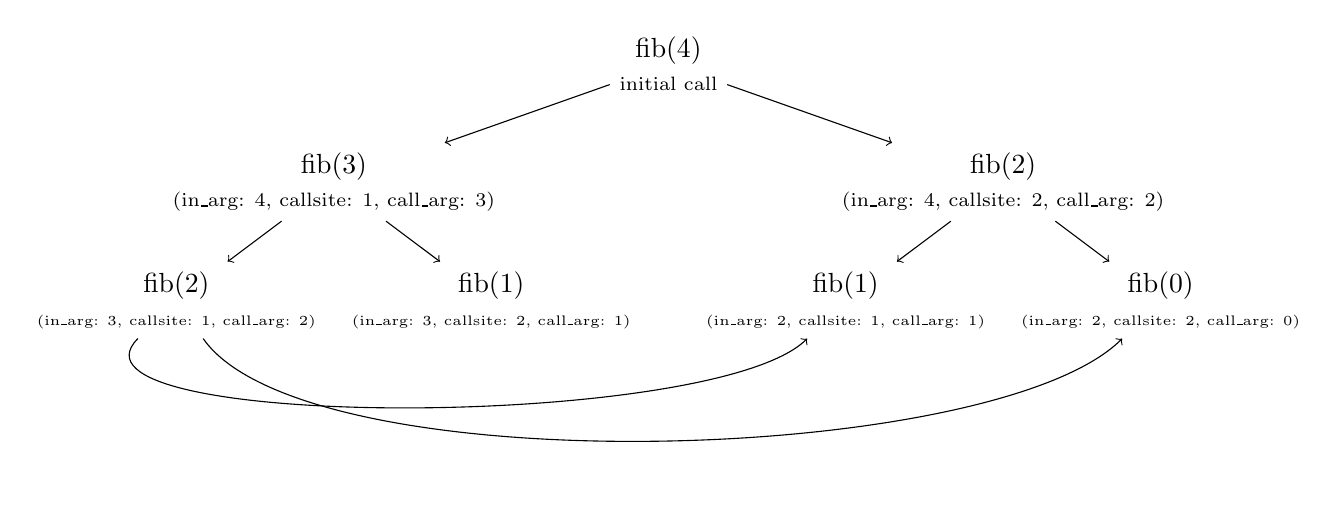
\begin{tikzpicture}[->, level distance=15mm, align=center]
\tikzstyle{level 1}=[sibling distance=85mm]
\tikzstyle{level 2}=[sibling distance=40mm]
\tikzstyle{level 3}=[sibling distance=40mm]
\node{fib(4)\\\scriptsize{initial call}}
  child { node {fib(3)\\\scriptsize{(in\_arg: 4, callsite: 1, call\_arg: 3)}}
    child {node (fib2) {fib(2)\\\tiny{(in\_arg: 3, callsite: 1, call\_arg: 2)}}
      %child {node {fib(1)\\\tiny{(in\_arg: 4, callsite: 2, call\_arg: 2)}} }
      %child {node {fib(0)\\\tiny{(in\_arg: 4, callsite: 2, call\_arg: 2)}} }
    }
    child {node (fib1) {fib(1)\\\tiny{(in\_arg: 3, callsite: 2, call\_arg: 1)}} }
  }
  child {node {fib(2)\\\scriptsize{(in\_arg: 4, callsite: 2, call\_arg: 2)}}
    child {node (fib1) {fib(1)\\\tiny{(in\_arg: 2, callsite: 1, call\_arg: 1)}} }
    child {node (fib0) {fib(0)\\\tiny{(in\_arg: 2, callsite: 2, call\_arg: 0)}} }
  };
\draw[->, bend left=10, out=225, in=225, looseness=0.5] (fib2) edge (fib1);
\draw[->, bend right=5, out=305, in=225, looseness=0.5] (fib2) edge (fib0);
\end{tikzpicture}

\begin{tabular}{c|c|c}
\texttt{in\_1} & \texttt{callsite} & \texttt{arg\_1} \\
\hline
\hline
\textcolor{red}{4} & 1 & \textcolor{green}{3} \\
\textcolor{red}{4} & 2 & \textcolor{blue}{2} \\
\hline
\textcolor{green}{3} & 1 & 2 \\
\textcolor{green}{3} & 2 & 1 \\
\hline
\textcolor{blue}{2} & 1 & 1 \\
\textcolor{blue}{2} & 2 & 0 \\ 
\end{tabular}


How does the translation work? The first step, the scenario analysis, extracts all possible execution scenarios of a given function. For the Fibonacci UDF given above, the output of the inference rules is the following:\\

As we can see, the \CASE-expression is deconstructed. Note that the predicates resemble exactly the program flow of the \CASE-expression: A \THEN-branch is only evaluated if all leading \WHEN-expressions evaluated to false and the current predicate evaluates to true. The predicate of the \ELSE-branch is just the negation of all previous predicates.



Based on the recursive scenarios, all callsites are enumerated and their arguments extracted to self-contained queries. The recursive cases are enriched with a list of callsites they contain to check later on whether a result for all callsites of an recursive scenario is present yet.
  Callsite 1: (Argument 1: SELECT \$1 - 1) 
  Callsite 2: (Argument 1: SELECT \$1 - 2)
  
Now we have all the data required to construct a query that assembles the callgraph. This is achieved by recursivly collecting the arguments of the callsites of those scenarios that occur under the given input argeters. In the beginning, the original input argeters of the function are used. As we recurse, we iterate through the newly added callsite arguments to collect data of further calls. We end up by a relational encoding of a callgraph.

\sqlcode{snippets/fib_discovery.sql}

, tracking calls down to the basecases (ie. the nonrecursive scenarios) without evaluating anything from the original function except the callsite-arguments. After the creation of the callgraph, we know the input argeters for the basecases and can evaluate them. With the results of the basecases at hand, it is now possible to continue evaluation up the callgraph. For each recursive scenario we check if for all contained callsites with the given input arguments, a result already exists. If so, the call in the recursive scenario is replaced with the reference to the result and the recursive scenario can be evaluated.

% What are the key components of my approach and results? Also include any specific limitations. 
The translation of an UDF is split in two major parts, static analysis and template expansion. During static analysis the original UDF is split into different evaluation scenarios with a predicate under that this scenario will be evaluated. The analysis result is used to choose and fill appropriate templates to build the translated function.

\paragraph*{Static analysis}
%Case analysis: 
%Callsite extraction
%Recursion type detection
%Constant argeter detection
%Hashability checks
This thesis goal is to extend to range of algorithms for which it is easy to write a fairly performing implementation in standard SQL. I provide inference rules to perform a syntax directed analysis of a given SQL UDF that extracts evaluation scenarios alongside with conditions under which each scenario is executed. To analyze the query correclty, it is necessary to track direct and indirect references to callsites while analyzing the query. Callsites are tracked through FROM, subqueries and CTEs and also takes shadowing into account. Extracted scenarios also contain only actually referenced CTEs, deleting unused CTEs that were referenced by other WHEN-branches. The extracted predicates do not contain any callsites so that they can be used to guard the execution of the scenarios. Predicates, Scenarios and Callsite arguments are extracted in a closed form, so that they contain no free variables and can be evaluated independenty from each other. To achieve this, none of these may reference a row-variables from an outside FROM, only table-variables may be referenced, including outside CTEs. This also limits the ability of the UDF to perform meaningful computations that return tabular results, which we forbid entirely for now.

Each scenario is generated from the different branches of a \CASE-statement and the predicates that need to be fulfilled to reach a given \WHEN-branch. Each resulting scenario is semantically equivalent to the original query if its predicate is fulfilled. All scenarios combined are semantically equivalent to the original query. The scenarios are divided into basecases, that do not contain any recursive callsites, and recursive cases that do contain one or more callsites. Some more analysis is performed on the generated scenarios to detect properties of the function like tail recursion.



\paragraph*{Template-based translation}
%Callstack
%Basecases
%TerminationCheck
%Evaluation
From the extracted data an appropriate template is filled, forming the translation. The translation utilizes the iterative nature of WITH RECURSIVE to implement an actual iterative version of the recursive UDF. First, the callstack is discovered by iterativly collecting the new arguments of the callsites in the appropiate scenario. Second, the basecases are evaluated and all new computable results are collected. This repeats until the final result is computed. Cases where the translation would terminate but the original does not are detected and an infinite loop is created to mimic the original behaviour.

The translation template consists of a discovery-phase and an evaluation-phase. During discovery the callstack is built, collecting all recursive calls down to the nonrecursive basecases. From the discovery-table it is now possible to look up the input arguments that lead to a nonrecursive scenario which can be used to begin the recursive evaluation process. As soon as results for all callsites of a given scenario exist, this scenario can be evaluated. The query continues recursively until the argeter of the original call is found in the evaluation table.
    

\paragraph*{Results}
Static analysis is flexible, limitations sound hard, but are not so bad. Generalization to other conditionals is easy possible, implementation is well structured in phases and easy expandable.

The translation is many magnitudes faster than the original naive recursive function. The original fib-function can be called with max fib(23), while the translation handles still fib(100) within ca. 300ms on the same machine. Problem specific optimized solutions still always wins.

\paragraph*{Thesis overview}
First I will establish the backgrounds required for this thesis. The evaluation of SQL-queries, which is important to understand query performance, is covered first. Special focus is laid on the evaluation of WITH RECURSIVE which we utilize to create a translation from a recursive to an actually iterative function. The evaluation of SQL-UDFs is covered then, showing differences in evaluation that lead to the poor performance of recursive UDFs. Important forms of recursion, as well as pros and cons are dicussed afterwards. The background-chapter closes with a short primer on Small step Operational Semantics.

Before I present the rules in depth, I first introduce a couple of preliminaries are necessary to introduce simplyfying notations ans specify constraints on the functions that can be translated.
...